%=== Préambule ===========================================================

\documentclass{beamer}
\usepackage{pdfpages}
\usepackage[english]{babel}
\usepackage{xspace}
\usepackage{pifont}
\usepackage{hyperref}
\usepackage{listings}
\usepackage{csquotes}
\usepackage{graphicx}
\usepackage{animate,media9} %,movie15}
\usepackage{wrapfig}
\usepackage{pdfpages}
\usepackage{tikz}
\usepackage{natbib}
\uselanguage{English}
\usepackage{fontawesome5}
\languagepath{English}
\setcounter{tocdepth}{1}
\usepackage{setspace}
\usepackage{amsmath}
\def\glasses{{\sffamily 
\leavevmode\rlap{%
\rotatebox[origin=tr]{125}{J}\kern1ex%  
\rotatebox[origin=tr]{125}{J}}% 
\rotatebox[origin=c]{-90}{D}%   
\rotatebox[origin=c]{-90}{D}}%
\def\ialy{\sffamily 
\resizebox{1ex}{1.5ex}{\reflectbox{\rotatebox[origin=]{75}{J}}}\kern-1pt%
\rlap{\tiny$\ ^\bullet\kern2.5pt^\bullet$ }%
\rotatebox[origin=c]{-90}{D}%   
\rotatebox[origin=c]{-90}{D}\kern-1pt%  
\resizebox{1ex}{1.5ex}{\rotatebox[origin=]{75}{J}}}}


\lstset{
  numbers=left,
  basicstyle=\tiny\ttfamily,      
  breaklines=true, 
  showtabs=false,
  showstringspaces=false,
}  

%=== Configuration de Beamer et du thème metropolis ======================
\usepackage{bbding}
\usetheme[background=light]{metropolis}
\usepackage[clock]{ifsym}

\definecolor{mLightBrown}{HTML}{000000}
\definecolor{black}{HTML}{000000}
\setbeamercolor{structure}{fg=black,bg=mLightBrown}
\setbeamercolor{palette primary}{%
	use=normal text,
	fg=normal text.bg,
	bg=mLightBrown
}
%\setsansfont[BoldFont={Linux Libertine G Bold},Numbers={OldStyle}]{Linux Libertine G}

\metroset{block=fill}

%=== Page de titre =======================================================

%path to logo and biblio -> to be adapted to your local directories 
\newcommand\dirlogo{../../../../logos/}
\newcommand\dirbiblio{../../../../biblio}



\title{{\normalsize \vskip 2cm 
Taller 1: Problemas inversos}}
\subtitle{\small Y un poco de programación}
\author{Hugo S\'anchez-Reyes \\ {\tiny Charg\'e de Recherche, Institut de Recherche pour le Développement IRD - ISTerre} \\ 
\\
\\
Gracias a mis colaboradores, \\
Romain Brossier, Ludovic Métivier \\
\\
Gracias al IGP por recibirme
}


\date[2021]{\vskip -0.5cm \hfill 12 Janvier 2023}

\subject{Group Meeting}

\titlegraphic{\centering \vspace{-15pt}
\includegraphics[height=1.3cm]{\dirlogo/logo_seminar_2022.pdf} \par} %\qquad  
\includegraphics[height=1.4cm]{../../logos/anr_eqtime.png} \par }


\addtobeamertemplate{frametitle}{}{%
\begin{tikzpicture}[remember picture,overlay]
  \node[anchor=north east,yshift=0.0ex] at (current page.north east) {
\includegraphics[height=4ex]{\dirlogo/IRD_neg.png}};
  %\node[anchor=north east,yshift=0.5ex] at (current page.north east) {\includegraphics[height=3.3ex]{\dirlogo/seiscope_color_light_background}};
\end{tikzpicture}}



%=== Document ============================================================

\begin{document}

% --- Préambule ---------------------------------------------------------------

\begin{frame}
    \titlepage
\end{frame}


\begin{frame} {Objectivos de este taller}

\begin{itemize}
 \item What is inversion? When do we meet this class of problem
(inversion is everywhere in physical, sociological, health, \dots )
 \item Provide recipes to solve linear inverse problems
 \item Give simple examples
 \item Two useful books on the subject, and main credits:
 \begin{itemize}
  \item[1] Geophysical Data Analysis: Discrete Inverse Theory (Revised Edition) William Menke (1989), Academic Press
  \item[2] Parameter Estimation and Inverse Problems (Second Edition) Richard C. Aster, Brian Borchers \& Clifford H. Thurber (2013), Academic Press
 \end{itemize}
\end{itemize}
 
\end{frame}

\begin{frame}
 {Outline}
 
 \tableofcontents

\end{frame}

\section{Mathematical background}

\begin{frame}
 {Forward and inverse problems}

Forward problem: \\
Model parameters $\rightarrow$ Forward modeling $\rightarrow$ Predicted data \\
Inverse problem: \\
Observed data $\rightarrow$ Inverse modeling $\rightarrow$ Parameter estimation

\end{frame}

\begin{frame}
 {Principios matemáticos}
 
 We are interested in the relationships between physical (or chemical, economic, \dots) model parameters $m$ and a set of data $d$.
 
 \begin{itemize}
  \item We assume a good knowledge of the laws governing the investigated phenomena (underlying physics), in the form of a function G such that
  \begin{equation}
   d = G (m )
  \end{equation}
  \item In the mathematical model $d = G(m)$, the forward modeling operator $G$ can be defined as
  \begin{itemize}
   \item a linear or nonlinear system of algebraic equations
   \item the solution of an ODE or PDE
  \end{itemize}
  \item Forward problem: find $d$ given $m$
  \item Inverse problem: find $m$ given $d_c$
  \item Model identification problem: find $G$ knowing some values of $d$ and $m$
 \end{itemize}
 
\end{frame}


\begin{frame}
 {Ejemplos:}
 
 \begin{center}
  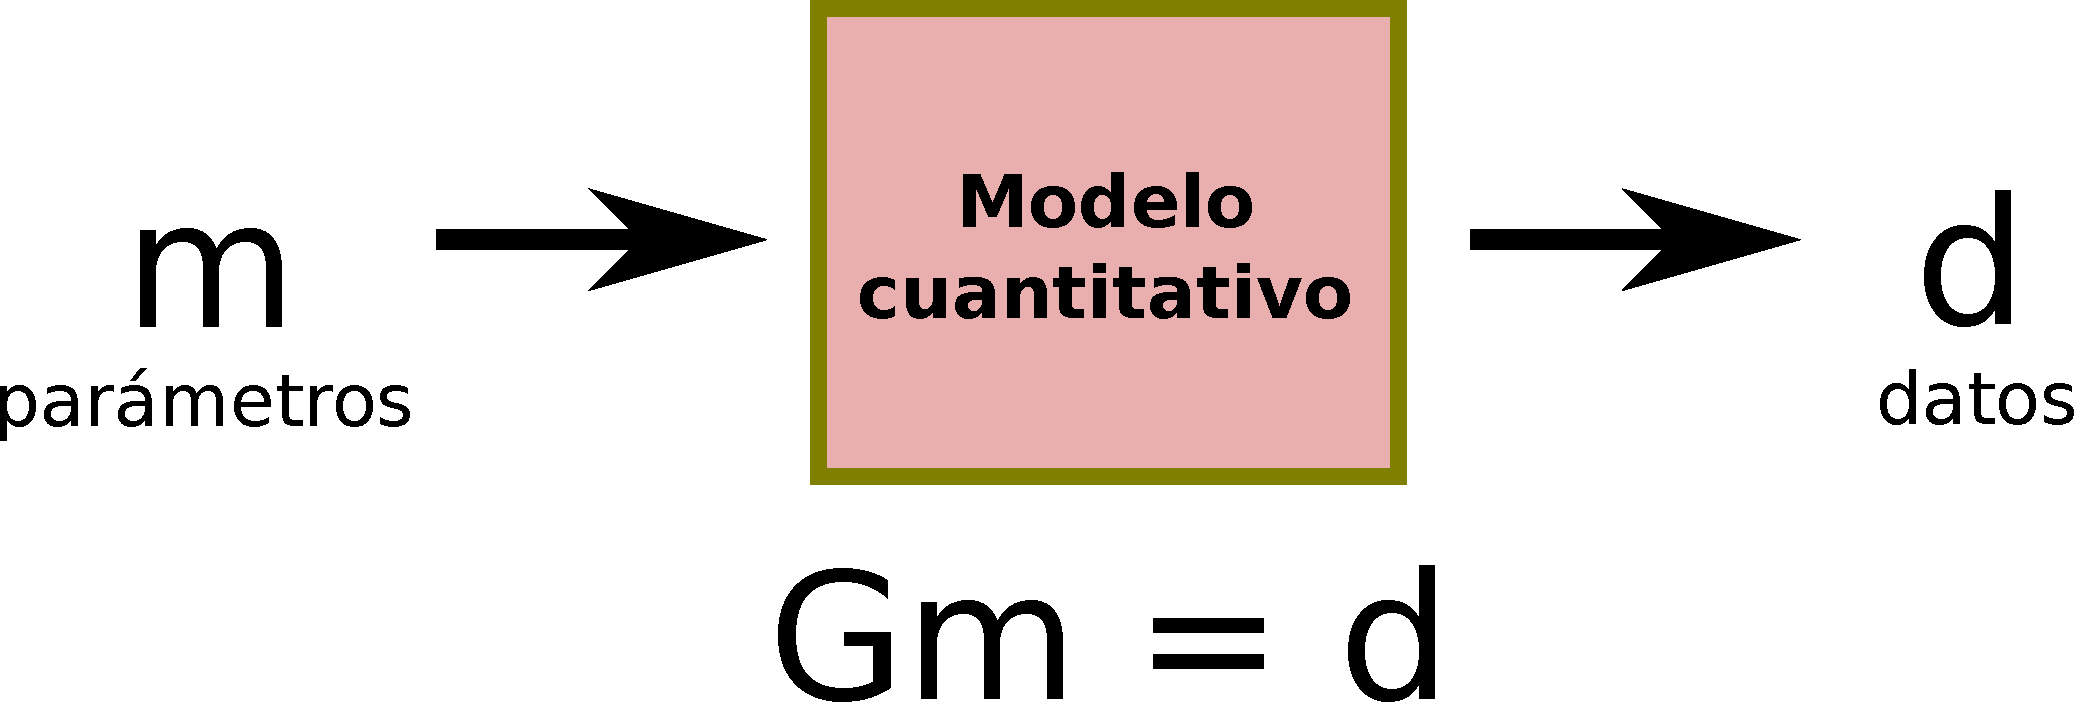
\includegraphics[width=0.6\linewidth]{images/forward.pdf}  
 \end{center}
 \begin{minipage}{0.45\linewidth}
 \begin{center}
  Modelo $\rightarrow$ línea recta \\
 \end{center}
 ejemplo:
 \begin{align*}
  T_1 = & a + bt_1 \\
  T_2 = & a + bt_2 \\
  \vdots \\
  T_N = & a  + bt_N
 \end{align*}
 \end{minipage}
 \begin{minipage}{0.45\linewidth}
  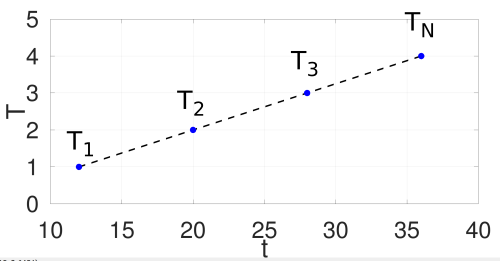
\includegraphics[width=1\linewidth]{images/line.png}
 \end{minipage}
 
\end{frame}

\begin{frame}
 {Ejemplos:}
 
 \begin{center}
  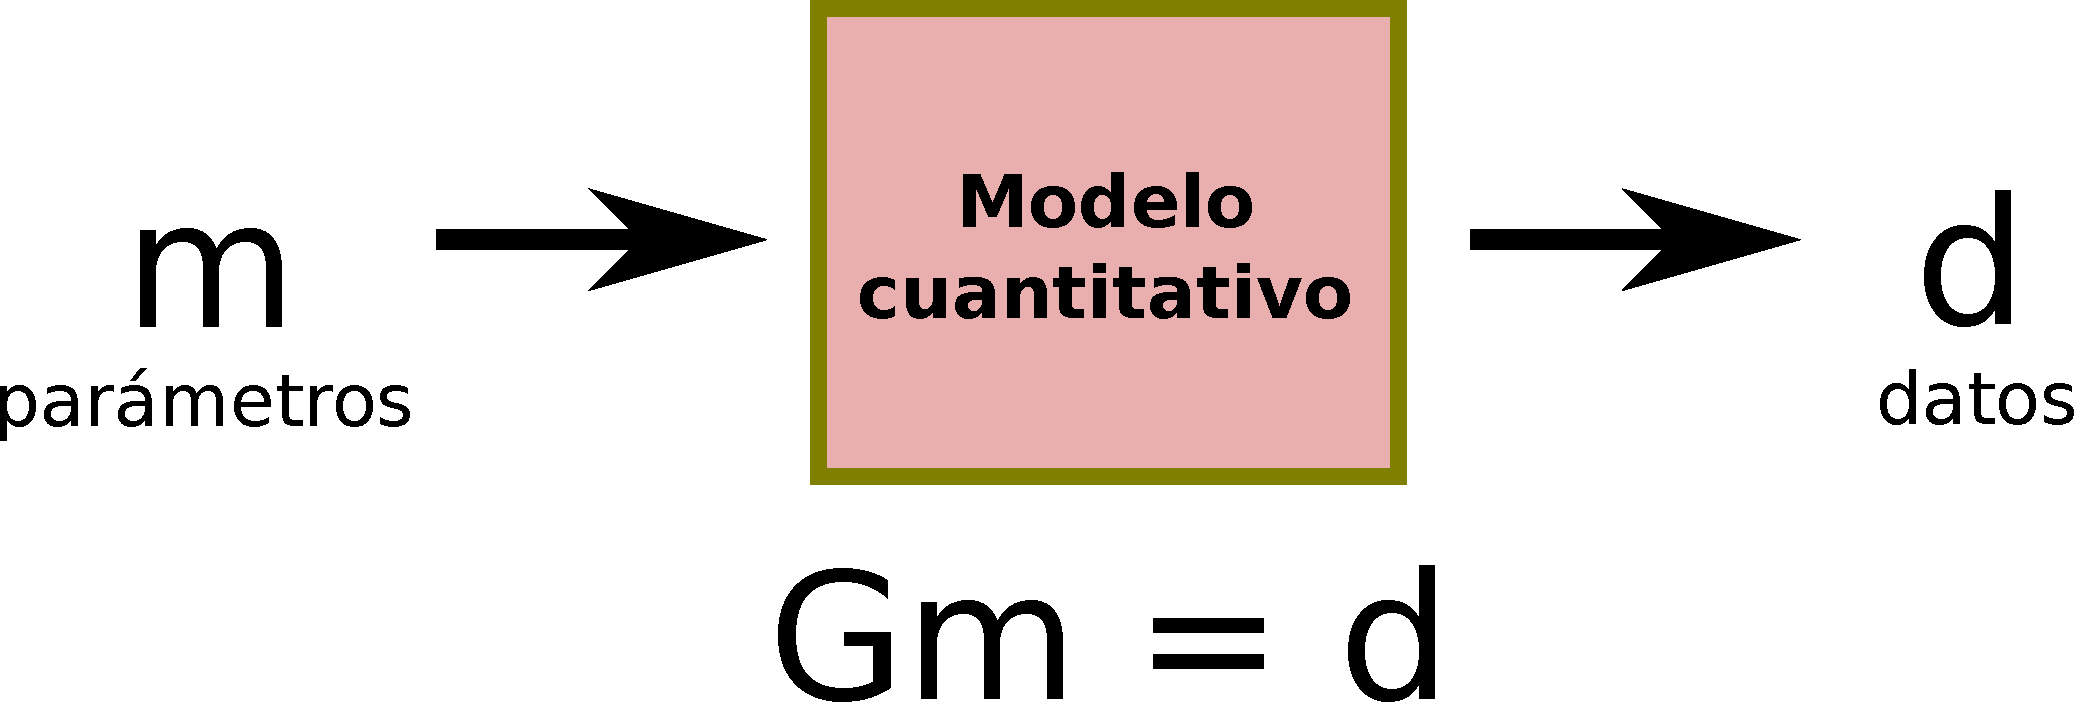
\includegraphics[width=0.6\linewidth]{images/forward.pdf}  
 \end{center}
 \begin{minipage}{0.45\linewidth}
 \begin{center}
  Modelo $\rightarrow$ línea recta \\
 \end{center}
 ejemplo:
 \begin{align*}
  T_1 = & a + bt_1 \\
  T_2 = & a + bt_2 \\
  \vdots \\
  T_N = & a  + bt_N
 \end{align*}
 \end{minipage}
 \begin{minipage}{0.45\linewidth}
 en algebra lineal:
  \begin{equation*}
   \begin{bmatrix}
    T_1 \\
    T_2 \\
    \vdots \\
    T_N
   \end{bmatrix}
   = 
   \begin{bmatrix}
    1 & t_1 \\
    1 & t_2 \\
    \vdots & \vdots \\
    1 & t_N
   \end{bmatrix}
   \begin{bmatrix}
   a \\
   b
   \end{bmatrix}
 \end{equation*} 
  \begin{equation*}
  \underline{d} = \underline{\underline{G}} \underline{m}
 \end{equation*} 
 \end{minipage}
 
\end{frame}

\begin{frame}
 {Ejemplos:}
 
 \begin{center}
  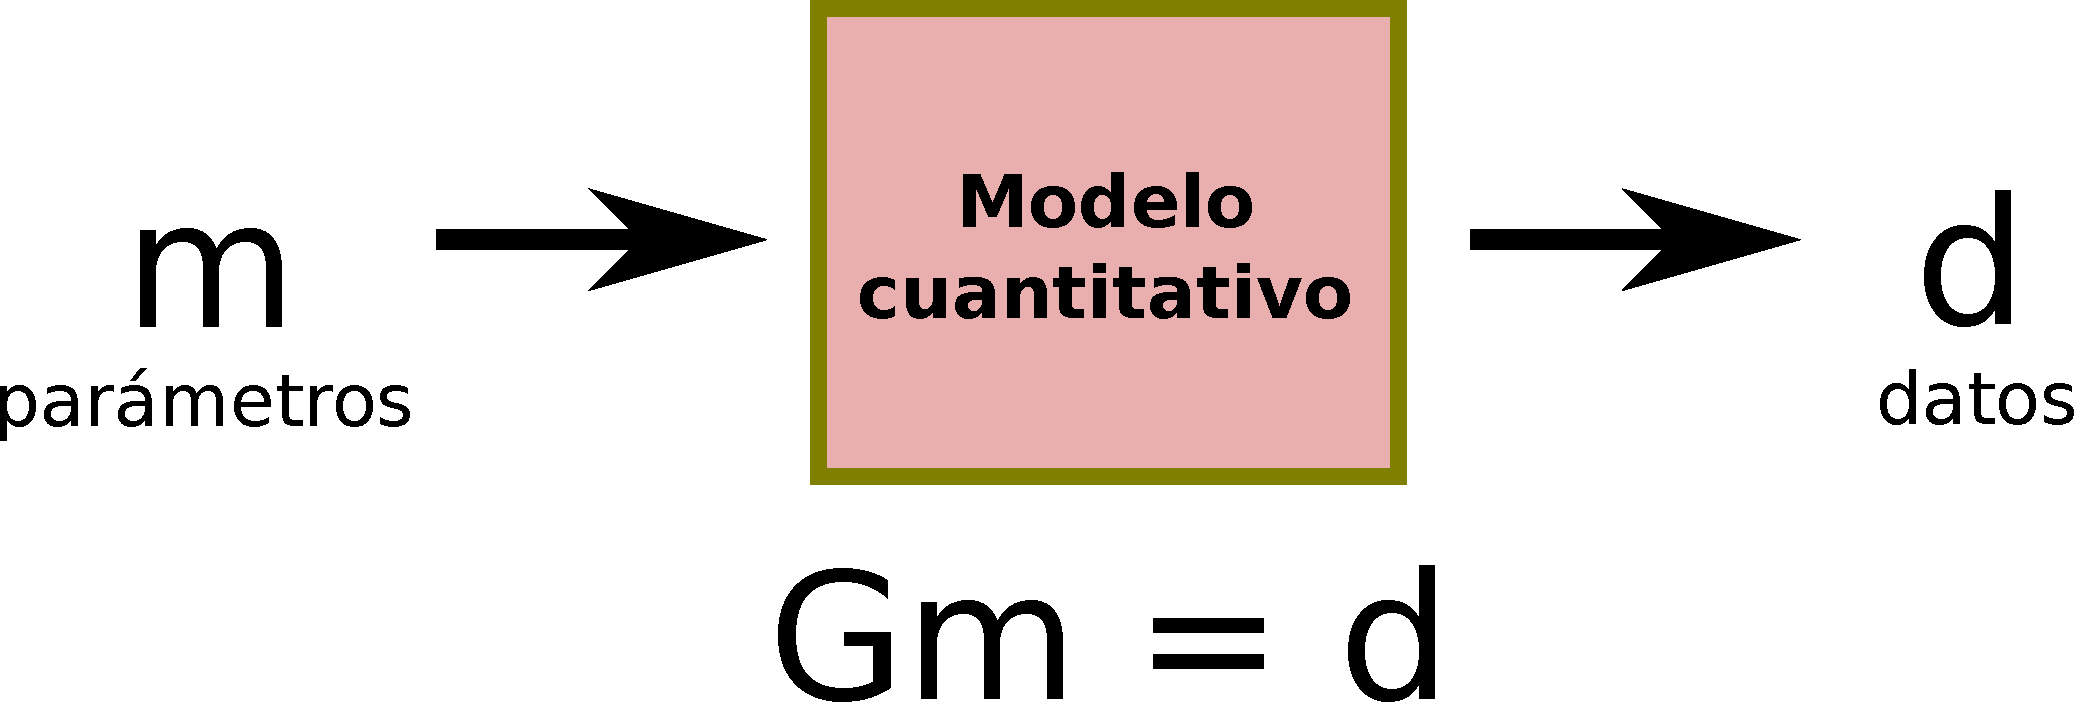
\includegraphics[width=0.6\linewidth]{images/forward.pdf}  
 \end{center}
 \begin{minipage}{0.45\linewidth}
 \begin{center}
  Modelo $\rightarrow$ línea recta \\
 \end{center}
 ejemplo:
 \begin{align*}
  T_1 = & a + bt_1 \\
  T_2 = & a + bt_2 \\
  \vdots \\
  T_N = & a  + bt_N
 \end{align*}
 \end{minipage}
 \begin{minipage}{0.45\linewidth}
 en algebra lineal:
  \begin{equation*}
   \begin{bmatrix}
    T_1 \\
    T_2 \\
    \vdots \\
    T_N
   \end{bmatrix}_{[N\times1]}
   = 
   \begin{bmatrix}
    1 & t_1 \\
    1 & t_2 \\
    \vdots & \vdots \\
    1 & t_N
   \end{bmatrix}_{[N\times2]}
   \begin{bmatrix}
   a \\
   b
   \end{bmatrix}_{[2\times1]}
 \end{equation*} 
  \begin{equation*}
  \underline{d} = \underline{\underline{G}} \underline{m}
 \end{equation*} 
 \end{minipage}
 
\end{frame}





\section{Inverse problem (and/or optimization) specific notions}

\begin{frame}
 {Why inverse problem are difficult?}

 \begin{itemize}
  \item We are concerned with far more than just finding an acceptable model {$m_i$} that fits the data {$d_i$} , assuming a physical model $G$.
  \item There may be several acceptable solutions
  \item Essential issues are i) solution existence, ii) solution uniqueness and iii) instability of the solution process
   \item There may be no model that exactly fits the data
   \begin{itemize}
    \item The model is wrong, or approximate
    \item Data are noisy
   \end{itemize}
   \item  Rank deficiency in the model space; null space= a set of parameter combination that do not change the data: $d=G(m+lambda*m0)$ => model resolution analysis because the solution may be biased with respect to the reality
 \item[ii)] Several solutions can fit equally the same dataset: \\ in potential field, several density distribution produce the same gravity field
 \item[iii)] Instability of the inverse calculation: small changes in data can lead to huge changes in model: Ill-posed or in lthe linear case: Ill-conditionned. To solve this one add additional constraints that stabilize the computation but biases the solution
 \end{itemize}




 
\end{frame}



\section{The linear case}

\end{document}

